%\documentclass{article}
\documentclass[12pt]{article}
\usepackage{fontspec}
\usepackage{graphicx}
\usepackage{subcaption}
\setmainfont{Times New Roman}
\renewenvironment{abstract}
  {\quotation}
  {\endquotation}
  
\usepackage[a4paper, margin=2.5cm]{geometry}

% Language setting
% Replace `english' with e.g. `spanish' to change the document language
\usepackage[english]{babel}
\usepackage{pdflscape}
\usepackage{booktabs}
\usepackage{caption}
% Set page size and margins
% Replace `letterpaper' with `a4paper' for UK/EU standard size
%\usepackage[letterpaper,top=2cm,bottom=2cm,left=3cm,right=3cm,marginparwidth=1.75cm]{geometry}
\usepackage{threeparttablex}

% Useful packages
\usepackage{titlesec}
\usepackage{amsmath}
\usepackage{graphicx}
\usepackage[colorlinks=true, allcolors=black]{hyperref}
\usepackage{booktabs} % Required for \toprule, \midrule, \bottomrule
\usepackage{multirow}
\usepackage{tabularx}
\usepackage{caption}
  \usepackage[labelfont=bf]{caption}
\usepackage{tablefootnote}
\usepackage{fancyhdr}   % For custom headers and footers
\usepackage[backend=biber, style=authoryear, urldate=comp, url=true, doi=false, isbn=false]{biblatex}
\addbibresource{igvz.bib} % Replace 'yourbibfile.bib' with your actual file name

\usepackage{lastpage}  % To get the label of the last page
\pagestyle{fancy}
\fancyhf{} % clear all header and footer fields
\fancyfoot[C]{Page \thepage\ of \pageref{LastPage}}  % Center footer
\renewcommand{\headrulewidth}{0pt}  % Optional: removes the horizontal line in the header

% Setting up the page style for landscape with vertical page numbers
\fancypagestyle{landscape}{
    \fancyhf{} % Clear all header and footer fields
    \fancyfoot[C]{ % Center footer
        \begin{rotate}{90} % Rotate text for vertical alignment
            \thepage % Page number
        \end{rotate}
    }
    \renewcommand{\headrulewidth}{0pt} % No header rule
    \renewcommand{\footrulewidth}{0pt} % No footer rule
}

% Customizing section headers
\titleformat{\section}
  {\normalfont\small\bfseries}{\thesection}{1em}{}
\titlespacing*{\section}{0pt}{1ex plus 1ex minus .2ex}{1ex plus .2ex}

\titleformat{\subsection}
  {\normalfont\small\bfseries}{\thesubsection}{1em}{}
\titlespacing*{\subsection}{0pt}{1ex plus 1ex minus .2ex}{1ex plus .2ex}

\titleformat{\subsubsection}
  {\normalfont\small\bfseries}{\thesubsubsection}{1em}{}
\titlespacing*{\subsubsection}{0pt}{1ex plus 1ex minus .2ex}{1ex plus .2ex}

\begin{document}

\centerline{\textbf{ }}
\newpage

\centerline{\textbf{Abstract}}

\noindent \textbf{Objective: }Maternal morbidity and perinatal mortality are relatively higher among pregnant asylum seekers than that of the host population. Interactive group education is a promising method to improve knowledge levels. This study aims to assess the impact of interactive group education sessions on pregnant asylum-seeking women's knowledge of the Dutch maternity care system, pregnancy patho-physiology, childbirth, postpartum care, and to explore its effect on satisfaction of care.\\
\noindent \textbf{Methods}: Pregnant asylum seekers at AZC, Ter Apel were divided into intervention and control groups. The intervention group received two interactive sessions and was assessed by a validated knowledge questionnaire. Patient satisfaction was observed using the LADY-X questionnaire. Demographics, knowledge scores, and LADY-X responses were analyzed.\\
\noindent \textbf{Results:} Demographics were similar between groups (parity: p=0.39, gravidity: p=0.61, gestational age: p=0.14). Both groups had comparable median scores at T1 (intervention: 9, control: 10), with varying ranges (intervention: 0-16, control: 4-15). By T2, the intervention group showed an improvement in scores compared to the control group (median difference: 3, range: -13 to 17; p=0.013). No statistical analysis could be conducted on LADY-X questionnaire responses due to participant relocations.\\
\noindent \textbf{Conclusion: }The interactive group education had a positive impact on knowledge levels compared to regular care offered in the Netherlands on pregnant asylum-seekers in AZC, Ter Apel. Due to constant relocations, no statistical analysis was able to be performed on patient satisfaction, highlighting the unstable circumstances pregnant asylum-seekers. \\

\centerline{\textbf{Samenvatting}}
\noindent \textbf{Doelstelling}: Maternale morbiditeit en perinatale mortaliteit liggen relatief hoger onder zwangere asielzoekers dan onder de autochtone bevolking. Interactieve groepseducatie is een veelbelovende methode om kennisniveaus te verbeteren. Dit onderzoek observeert de impact van interactieve groepseducatiesessies op de kennis van zwangere asielzoekers over het Nederlandse verloskundige zorg, de (patho)fysiologie van de zwangerschap, bevalling, postpartumperiode en om het effect ervan op tevredenheid over de zorg te onderzoeken.\\
\noindent \textbf{Methoden}: Zwangere asielzoekers in AZC, Ter Apel werden verdeeld in interventie- en controlegroepen. De interventiegroep kreeg twee interactieve sessies wat werd geëvalueerd met een gevalideerde kennisvragenlijst. Patiënttevredenheid werd gemeten met behulp van de LADY-X vragenlijst. Demografische gegevens, kenniscores en LADY-X-reacties werden geanalyseerd.\\
\noindent \textbf{Resultaten}: Demografische kenmerken waren vergelijkbaar tussen de groepen (pariteit: p=0.39, graviditeit: p=0.61, zwangerschapsduur: p=0.14). Beide groepen hadden vergelijkbare mediane kennisscores bij T1 (interventie: 9 punten, controle: 10 punten), met variërende bereiken (interventie: 0-16, controle: 4-15). Bij T2 vertoonde de interventiegroep een verbetering in kennisscores vergeleken met de controlegroep (mediaan verschil: 3, bereik: -13 tot 17; p=0.013). Vanwege relocaties van deelnemers kon er geen statistische analyse worden uitgevoerd op de LADY-X vragenlijst\\
\noindent \textbf{Conclusie}: De interactieve groepseducatie had een positief effect op het kennisniveau in vergelijking met de standaard zorg die in Nederland wordt aangeboden aan zwangere asielzoekers in het AZC, Ter Apel. Vanwege voortdurende relocaties en door ontbrekende deelnemers kon er geen statistische analyse worden uitgevoerd op patiënttevredenheid, wat de onstabiele omstandigheden waarin zwangere asielzoekers zich bevinden benadrukt. \\

\newpage
%\centerline{\textbf{ }}
\tableofcontents

\newpage
\section{Introduction}
\noindent According to the 2022 population statistics, the Dutch population consisted of 17.6 million people, of which 2.6 million (15\%) were born abroad. Of these, the first-migration immigrants were approximately 200,000 (7.7\%) were considered refugees under the UNHCR mandate (1-2). In the same year, the number of asylum seekers who applied for asylum in the Netherlands for the first time peaked since 2015 (3). In 2023, the most common nationalities amongst asylum-seekers were Syrian, Turkish and Eritrean with an increase of 72\% since 2022 (4). \\

\noindent About 25\% of the asylum-seeking women are of reproductive age and a significant proportion are pregnant or become pregnant during the time they seek refuge (2). A considerable portion of female refugees who are pregnant and anticipated to give birth during their time in the Netherlands (5). \\

\noindent Studies indicate that pregnant asylum seekers experience significantly higher rates of maternal mortality and morbidity (6,7). Also, perinatal mortality is two times higher in pregnant asylum seekers as compared to Dutch women (8). Currently, pregnant asylum seekers receive the same antenatal care as native Dutch women. However, various factors make it challenging to provide adequate prenatal care to asylum seekers. Studies have demonstrated that the utilisation of antenatal care services in the Netherlands is notably lower among ethnic minority groups compared to native women. Late initiation of prenatal care, in particular, reduces the time available to provide these women with adequate and sufficient information (9). \\

\noindent Factors contributing to the under-utilisation of antenatal care and complications during childbirth among ethnic minority groups in the Netherlands include inadequate understanding of the Dutch healthcare system, language barriers, lower educational levels, and the prevalence of unplanned or unwanted pregnancies. Amongst the asylum seekers, the transfer between refugee centers resulting in discontinuity of antenatal care adds to this (10). Providing antenatal care to asylum seekers, as opposed to Dutch nationals, requires a significant investment of time from caregivers. This is largely due to the language and cultural barriers, as well as the asylum seekers' limited familiarity with the Dutch healthcare system. \\

\noindent Pregnant asylum seekers may benefit from group healthcare, which involves health professionals delivering care and education to groups of individuals facing similar health issues, while also facilitating health assessments and peer support. Studies indicate that women who participate in group antenatal care experience fewer preterm births, gain more prenatal knowledge, and feel better prepared for labor and delivery (11). Group antenatal care significantly influences breastfeeding initiation post-delivery, with more women beginning to breastfeed after participating in such programs (11). Furthermore, these group settings provide a supportive environment where women can openly share their fears, concerns, and experiences, creating a sense of community and reducing feelings of isolation during pregnancy. This further facilitates the development of trusting relationships with their healthcare providers (12-14). Overall, group antenatal care is linked to improved clinical outcomes, higher maternal satisfaction scores, and greater overall satisfaction with prenatal care (11-15). \\

\noindent In the Netherlands, pregnant asylum seekers receive the same antenatal care as non-migrant women. Studies in Norway have indicated that perinatal mortality, maternal mortality, maternal morbidity, sudden infant death syndrome, prematurity, and low birth weight are disproportionately higher among non-western immigrants (16). These disparities suggest that traditional antenatal care may need to be adapted for asylum seekers, who often lack familiarity with the Dutch healthcare system and face language and cultural barriers that complicate care further. \\

\noindent Our study aims to assess the effectiveness of Interactive Group Education versus regular care in enhancing knowledge of the Dutch maternity care system, patho-physiology of pregnancy, childbirth, and the postpartum period among pregnant asylum seekers. Additionally, we aim to determine if these education sessions lead to increased satisfaction with care.

\section{Research Question}
Does participation in interactive group education sessions (IGVZ), compared to regular care, enhance knowledge levels among pregnant asylum seekers regarding the Dutch maternity care system, as well as the patho-physiology of pregnancy, childbirth, and the postpartum period and does it increase the satisfaction of care? 

\section{Methods}
\subsection{Data Sources}
This prospective-cohort study was conducted among pregnant asylum seekers at the asylum shelter in Ter Apel. 
Ter Apel is the only central location of the Centraal Orgaan Asielzoekers (COA; central asylum seeker organisation) in the Netherlands where asylum seekers entering the country are accommodated initially. COA is responsible for the reception, supervision and departure (from the reception location) of asylum seekers coming to the Netherlands. Within three days, identification, registration and tuberculosis (tbc) check-up takes place, after which individuals might be transferred to another processing location or remain in Ter Apel. The refugee center has a maximum capacity of 2000 people. \\

\noindent The study was carried out between 2017 and 2023. Interactive Group Education (IGVZ) for pregnant asylum seekers was offered in Ter Apel from February 2017 to December 2018, during which period, the project received funding from ZonMw (ZonMw; ZorgOnderzoek Nederland + Medical Sciences (Dutch abbreviation: MW). COA, the midwifery clinic in Ter Apel (NewLife), the hospital in Stadskanaal (Treant zorggroep), the municipal health service (GGD Groningen), the maternity care (Kraamzorg Groene Kruis) and advisory organisation ELANN (ELANN; Nascholing Ondersteuning Huisartsen) worked together to start this program. Interactive Group Education was offered to women with a gestational age of more than 34 weeks since they were not allowed to be transferred between refugee centers and will therefore be able to adhere to the meetings. After completion of the IGVZ project, only regular care was provided in Ter Apel due to lack of funding, while data collection for the control group continued until December 2023.
 
\begin{figure}
    \centering
    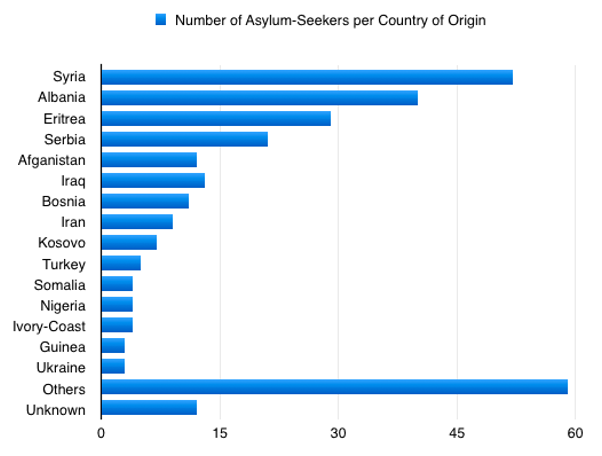
\includegraphics[width=0.5\linewidth]{bar-chart-country.png}
    \caption{Asylum-Seekers at Ter Appel (by Country of origin)}
    \label{fig:1}
\end{figure}

\subsection{Participant Demographics}
\subsubsection{Interactive Group Education program}

\noindent Women were enrolled in the Interactive Group Education if they were pregnant, asylum seekers in Ter Apel, had a gestational age of more than 34 weeks, and had been examined at the New Life midwifery practice. As many pregnancies did not have an exact term because they were not initially checked, an approximation of the gestational age was used. A female coordinator invited the pregnant women, planned the meetings and was present at each meeting. \\

\noindent The group antenatal care programme aimed to organise a total of three interactive group education sessions, but due to the constant relocation of asylum seekers, only two interactive group education sessions were eventually held, combining the information from the third and second session. During these sessions, the women were encouraged not only to listen but also to actively participate in discussions and activities that stimulated the learning process. The groups consisted of a minimum of 5 and a maximum of 10 women. Women attended these sessions without their partners. These sessions were held in addition to the regular midwife visits and  led by a registered (Dutch-speaking) midwife in combination with an official translator, who was also present while the participants were being administered the questionnaire. \\

\noindent All three sessions were to be led by the same group leaders. Interactive methods (group discussion, audio-visual support, anatomical models and interactive games) were used to transfer knowledge to the participants. During the sessions, there was time for group members to ask questions or interact with each other. The aim was to create a group feeling among the participants, so that ideally the interactive part would continue outside the sessions. It was taken into account that there might be a low level of education or a lack of basic knowledge about the human body among participants. Cultural, religious and language barriers were also considered by discussing customs and traditions from the participant's country. \\

\noindent During the first meeting, participants were introduced to the research and concept of the IGVZ by a midwife from a midwifery practice. After introductions between participants and meeting leaders, a 15-minute explanation of the Dutch obstetric care system followed. This explanation used a magnetic board with pictures to illustrate the system of regular antenatal care, the concept of male and female caregivers, accessibility of caregivers, and methods of contact. Information was also provided on medical examinations, lifestyle choices and diet (such as smoking, alcohol and drug use). Participants then engaged in interactive discussions focusing on personal and cultural preferences, experiences of antenatal care in their countries of origin, and their perspectives on the Dutch healthcare system. More technical issues such as transport, childcare during delivery, overnight stays with partners, referrals, what happens after 34 weeks, the COA money card and baby shopping lists were addressed by a COA staff member. This was followed by a discussion led by the midwife on a list of warning signs according to KNOV guidelines. Then, a 10-minute question and answer session ensued (Appendix 1). \\

\noindent The second session began by inviting participants to give feedback or ask questions about the previous session. Interactive examples were given by a midwife from a midwifery practice about who to contact during childbirth. An informative animated video about vaginal birth and pain relief was shown, followed by a more detailed demonstration using a mannequin, pictures, questions from participants and sharing of previous experiences. Topics such as induction of labour and caesarean section were also discussed by a midwife from the hospital using the above methods. Participants again discussed their own wishes and cultural practices, such as preferences for vaginal or caesarean birth, or experiences with induction of labour in their home countries compared to the Dutch healthcare system. A midwife gave interactive examples of who to contact during childbirth. A COA worker then briefly discussed transport, community registration, immunisation, and provided further information about children's health clinics and referrals. The midwife from the midwifery clinic also discussed postnatal care, explaining the role of a midwife during this period and discussing the use of medication. A maternity nurse gave insight into maternity care through an informative video, focusing on breastfeeding and bottle feeding. This was then followed by an interactive session where participants were given a platform to discuss common child health issues and potential breastfeeding challenges, followed by a breastfeeding demonstration. Later, a GGD health educator discussed topics related to sexuality, STDs and contraception, giving participants the opportunity to share their opinions and knowledge about contraception, STDs and gender in sexuality. Finally, participants were given 20 minutes to ask questions and give feedback. \\

\noindent The first session lasted 90 minutes, as the second and third session were combined, the second session lasted approximately 120 minutes with a break for participants (Appendix 1).

\subsubsection{Control group program}

\noindent Standard midwifery care in the control group at 34 weeks consisted of the following: individual check-ups at 34 weeks (routine check-up, blood pressure and external examination), 36 weeks (instructions and discussion about labour and delivery, blood pressure, external examination and, if indicated, an ultrasound scan for foetal position and biometry), 37, 38, 39, 40 weeks (blood pressure and external examination, answering questions about labour and delivery) and 41 weeks (discussion about due date and guidelines, ultrasound scan of amniotic fluid and rupture of membranes). \\
\noindent In order to facilitate comparison between the participants in the interactive education group sessions and the control group, individuals selected for the control group were demographically similar to those in the interactive group population. Specifically, the control group was carefully matched to the interactive group on the basis of criteria such as country of origin, gravidity and gestational age, preferably closely matching the gestational age of the IGVZ group participants, with a permissible difference of ±2 weeks if this was considered more optimal in terms of gestational age.

\subsection{Data collection}

\noindent Women were only included if they completed both knowledge questionnaires at the first and second meeting (T1 and T2). Participants did not have to be enrolled immediately on arrival at the AZC. They were eligible to participate even if they had been at the AZC for a longer period of time, as long as they met the inclusion criteria. \\

\noindent Data for the intervention group was collected between 2017 and 2018, and for the control group until December 2023. Data for the control group was collected after the IGVZ interactive education group sessions. The intention was to increase the knowledge among pregnant asylum seekers after the interactive group education, compared to before the interactive group education, and compared to the regular midwife visits on the following topics:the Dutch obstetric health care system, patho-physiology of pregnancy after 34 weeks, delivery and the postpartum period, alarm symptoms and appropriate contacts for each situation. This was measured by a knowledge questionnaire (Appendix 2) based on the TNO questionnaire of the Connect-In study evaluating the effects of Centering Pregnancy, with some additional questions about the KNOV alarm card and the Dutch obstetric health care system. Patient satisfaction was measured using the LADY-X questionnaire (Gärtner 2015, Appendix 3) (17-18).The questionnaires were translated into Arabic and Tigrinya by certified translators and were checked for appropriateness by a Syrian and an Eritrean physician. \\

\noindent These questionnaires were administered during a regular individual antenatal visit with the midwife before the start of the first session and at the end of the second session, as well as in the postpartum period. In the control group, questionnaires were intended to be administered between week 34, 36 and postpartum but were administered at varied times due to relocations. The questionnaires were administered amongst patients between their 17th week to 38th week of pregnancy. \\

\noindent The questionnaires took approximately 20 minutes to complete. The questionnaires were administered in the patient's own language, with the help of an interpreter if necessary. The knowledge questionnaires were administered at the beginning of the first session and at the end of the second session. 
Baseline characteristics were recorded: education, gravidity, parity, country of origin and gestational age at the first session. Women who were not able to complete all three sessions of the interactive group education because they did not attend or had a preterm birth were still included in the study. The number of these women was recorded. Participants who were unable to complete the questionnaires at the last session of the interactive group education were asked to complete the questionnaires after the birth, if possible. \\

\noindent This is measured by a knowledge questionnaire (Appendix 2) based on the TNO questionnaire of the Connect-In study evaluating the effects of Centering Pregnancy, with some additional questions about the KNOV-alarm card and the Dutch obstetric health care system. Patient satisfaction was measured using the LADY-X questionnaire (Gärtner 2015, Appendix 3) (17-18). \\

\noindent The questionnaires were translated into Arabic and Tigrinya by certified translators and were checked for appropriateness by a Syrian and an Eritrean physician. These questionnaires were administered during a regular individual antenatal visit with the midwife before the start of the first session and at the end of the second session, as well as in the postpartum period. In the control group, questionnaires were intended to be administered between week 34, 36 and postpartum but were administered at varied times due to relocations. The questionnaires were administered amongst patients between their 17th to 38th week of pregnancy. The questionnaires took approximately 20 minutes to complete. The questionnaires were administered in the patient's own language, with the help of an interpreter, when necessary. The knowledge questionnaires were administered at the beginning of the first session and at the end of the second session. 
\noindent Baseline characteristics were recorded: education, gravidity, parity, country of origin and gestational age in the first session. \\

\noindent Women who could not attend all three sessions of the interactive group education, either due to absence or preterm birth, were still included in the study, and their numbers were documented. Participants who failed to complete the questionnaires during the final session were given the opportunity to do so after giving birth, if possible.

\subsection{Ethical Considerations}

\noindent The ethical committee evaluated the study protocol as non-WMO (METC number: 2017/297 and UMCG research register number: 201700369). Participants received an identification number. These identification numbers were not based on the patient's initials or date of birth, but were numbered according to the order of receipt of the informed consent forms. A file containing the identification numbers of each participant was kept in a secure and encrypted individual file, stored on a hospital computer and accessible only to the principal investigators. The data was kept by the principal investigators for the duration of the proposed study and then stored in a registry at the University Medical Centre Groningen.

\subsection{Data analysis}

\textit{
\subsubsection{Sample Size Estimation}
}
\noindent A sample size calculation was performed using a one-tailed approach with an alpha level of 0.05, a standard deviation of 4.58 and a desired statistical power of 0.8. Taking into account the minimum effect size of clinical relevance, which was set at 2, the analysis yielded a minimum required sample size of 132 patients in total.
 \textit{
\subsubsection{Score System}
}
\noindent The knowledge questionnaires were checked for correct answers and scored accordingly; a correct answer was given a score of 1, an incorrect answer or "I don't know" was given 0 (zero) score.
 \textit{
\subsubsection{Estimate Normality Distribution }
}
\noindent The normality of the data was assessed using the Shapiro-Wilk test. Normally distributed continuous data was reported as mean ± SD, while not normally distributed continuous data was reported as median ± interquartile range (IQR). 
 \textit{
\subsubsection{Knowledge Questionnaire }
}
\noindent Non-parametric tests were performed to ensure that our statistical analyses were appropriate for the nature of the data when normality assumption was violated. The Wilcoxon test was used to compare knowledge questionnaire total scores between T1 and T2 (paired groups). Inter-group comparisons with IGVZ-group and control group were analysed through Mann-Whitney U test.
 \textit{
\subsubsection{Baseline Characteristics}
}
\noindent Descriptive statistics were used to identify baseline frequencies and characteristics within the participant cohort. Gravidity and parity were examined using the Chi-Contingency test. Gestational age distributions were examined using frequency analysis and the Mann-Whitney U test. Educational background was assessed using the Chi-Contingency test, while country of origin was examined using frequency analysis.

\textbf{
\section{Results}
}

\subsection{Demographics}

\noindent In this study, we enrolled a total of 130 participants, with 93 in the IGVZ intervention group and 37 in the control group. Baseline characteristics are shown in Table 1. We observed no significant statistical difference between the two groups regarding parity (p=0.39), gravidity (p=0.61), and gestational age (p=0.14). However, there was a notable variance in the range of gestational ages, with the IGVZ group presenting a broader span (median of 30 weeks, ranging from 5 to 40 weeks). This diversity could indicate varying entry points into the intervention stage of the program among participants. In contrast, the control group displayed a more constrained gestational age range (with a median of 31 weeks, ranging from 17 to 38 weeks). Additionally, there was a significant difference in educational background; notably, 40\% of the educational background data was missing from the IGVZ group. Demographically, participants predominantly originated from Nigeria, Syria, and Eritrea, comprising 38.7\%, 22.5\%, and 5.3\% of the IGVZ group, respectively, and 32.4\%, 27.02\%, and 8.1\% of the control group, respectively. 

\begin{figure}[htbp]
    \centering
    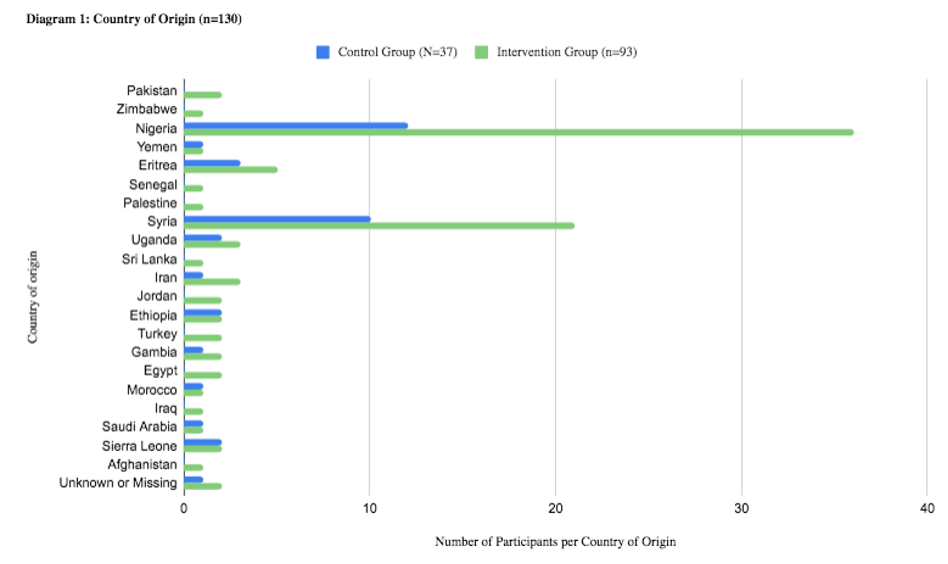
\includegraphics[width=\linewidth]{bar-chart.png} % Adjust the width as necessary
    \caption{Breakdown of Participants Per Country of Origin}
    \label{fig:bar-chart}
\end{figure}

\begin{figure}[htbp]
    \centering
    \begin{subfigure}{0.5\textwidth}
        \centering
        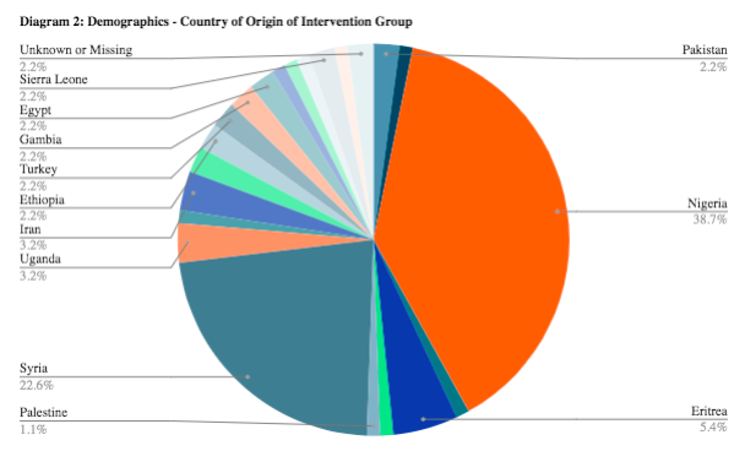
\includegraphics[width=\linewidth]{pie-chart-1.png} % Adjust the width as necessary
        \caption{Intervention Group}
        \label{fig:pie-chart-1}
    \end{subfigure}%
    \begin{subfigure}{0.5\textwidth}
        \centering
        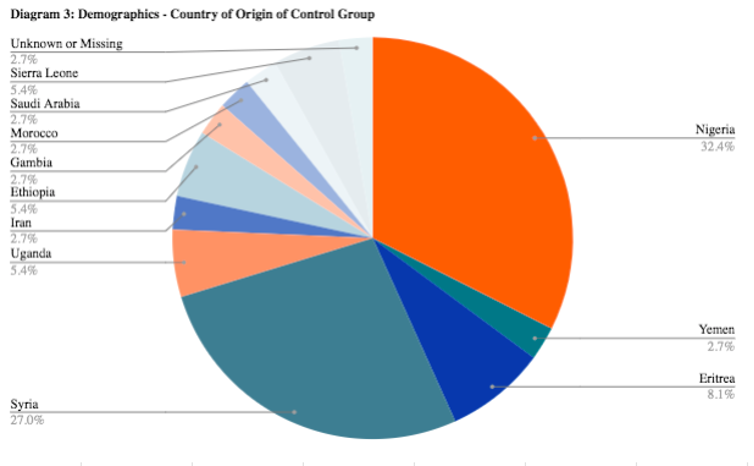
\includegraphics[width=\textwidth]{pie-chart-2.png} % Adjust the width as necessary
        \caption{Control Group}
        \label{fig:pie-chart-2}
    \end{subfigure}
    \caption{Comparative Analysis of Participant Origins}
\end{figure}

\captionsetup{justification=raggedright, singlelinecheck=false, skip=0pt, labelfont=bf}
\begin{table}[htbp]
    \caption{\textbf{Demographic Factors}}
    \begin{threeparttable}
        \small
        \begin{tabularx}{\textwidth}{>{\raggedright\arraybackslash}Xlll}
            \toprule
            \textbf{Baseline Characteristic} & \textbf{Intervention Group (n=93)} & \textbf{Control Group (n=37)} & \textbf{p-value} \\
            \midrule
            \textbf{Gravidity} &  &  &  \\
            \hspace{1em} Primigravida (1) & 32 (34.4\%) & 16 (43.2\%) & 0.61 \\
            \hspace{1em} Multigravida ($\geq$ 2) & 59 (63.4\%) & 20 (54.0\%) & -- \\
            \hspace{1em} NA\tnote{1} & 2 (2.1\%) & 1 (2.7\%) & -- \\
            \midrule
            \textbf{Parity} &  &  &  \\
            \hspace{1em} Nulliparous & 42 (45.1\%) & 13 (35.1\%) & 0.39 \\
            \hspace{1em} Multiparous & 51 (54.8\%) & 24 (64.8\%) & -- \\
            \midrule
            \textbf{Gestational Age (weeks)} &  &  &  \\
            \hspace{1em} $\textless{}$28 weeks & 40 (43.0\%) & 10 (27.0\%) & 0.14 \\
            \hspace{1em} 28-32 weeks & 14 (15.0\%) & 11 (29.7\%) & -- \\
            \hspace{1em} 32-37 weeks & 17 (18.2\%) & 15 (40.5\%) & -- \\
            \hspace{1em} 37-39 weeks & 11 (11.8\%) & 1 (2.7\%) & -- \\
            \hspace{1em} 39-41 weeks & 2 (2.1\%) & 0 (0\%) & -- \\
            \hspace{1em} $\textgreater{}$41 weeks & 9 (9.6\%) & 0 (0\%) & -- \\
            \midrule
            \textbf{Years of Education} &  &  &  \\
            \hspace{1em} 0-10 Years & 26 (27.9\%) & 21 (56.7\%) & 0.01 \\
            \hspace{1em} 11-15 Years & 15 (16.1\%) & 7 (18.9\%) & -- \\
            \hspace{1em} 16-20 Years & 12 (12.9\%) & 2 (5.4\%) & -- \\
            \hspace{1em} 21-25 Years & 2 (2.1\%) & 1 (2.7\%) & -- \\
            \hspace{1em} $\textgreater{}$25 Years or NA\tnote{1} & 38 (40.8\%) & -- & -- \\
            \bottomrule
        \end{tabularx}
        \begin{tablenotes}
            \footnotesize
            \item[1] Not Available
        \end{tablenotes}
    \end{threeparttable}
\end{table}

\begin{table}[htbp]
    \centering
    \captionsetup{justification=raggedright, singlelinecheck=false, skip=0pt, labelfont=bf}
    \caption{\textbf{Participants with Correct Knowledge Questionnaire Responses}}
    \begin{threeparttable}
        \small
        \begin{tabular}{ccccc}
            \toprule
            \textbf{Question} & \multicolumn{2}{c}{\textbf{T1}} & \multicolumn{2}{c}{\textbf{T2}} \\
            \cmidrule(lr){2-3} \cmidrule(lr){4-5}
            & \textbf{Intervention (n=93)} & \textbf{Control (n=37)} & \textbf{Intervention (n=93)} & \textbf{Control (n=37)} \\
            & 5.4\% Missing & 27\% Missing & 0\% Missing & 30\% Missing \\
            \midrule
            1 & 33 (37.5\%) & 16 (43.24\%) & 26 (28.89\%) & 12 (46.15\%) \\
            2 & 19* (21.59\%) & 9 (24.32\%) & 59* (69.41\%) & 9 (34.62\%) \\
            3 & 56* (63.64\%) & 25 (67.57\%) & 66* (76.74\%) & 17 (65.38\%) \\
            4 & 63* (71.59\%) & 23 (62.16\%) & 71* (85.54\%) & 19 (76\%) \\
            5 & 9* (10.23\%) & 3 (8.11\%) & 18* (21.69\%) & 4 (16\%) \\
            6 & 52 (59.09\%) & 22 (59.46\%) & 28 (33.73\%) & 11 (44\%) \\
            7 & 36* (40.91\%) & 23 (62.16\%) & 63* (75.9\%) & 14 (56\%) \\
            8 & 19 (21.59\%) & 8 (21.62\%) & 15 (18.07\%) & 2 (8\%) \\
            9 & 34* (38.64\%) & 9 (24.32\%) & 39* (46.99\%) & 10 (40\%) \\
            10 & 30* (34.09\%) & 11 (29.73\%) & 59* (71.08\%) & 11 (44\%) \\
            11 & 8* (9.09\%) & 10 (27.03\%) & 9* (10.84\%) & 8 (32\%) \\
            12 & 17* (19.32\%) & 8 (21.62\%) & 19* (22.89\%) & 15 (60\%) \\
            13a & 60* (68.18\%) & 27 (72.97\%) & 68* (81.93\%) & 23 (92\%) \\
            13b & 68* (77.27\%) & 35 (94.59\%) & 69* (83.13\%) & 22 (88\%) \\
            13c & 34* (38.64\%) & 16 (43.24\%) & 44* (53.01\%) & 13 (52\%) \\
            13d & 41* (46.59\%) & 17 (45.95\%) & 54* (65.06\%) & 13 (52\%) \\
            13e & 23* (26.14\%) & 16 (43.24\%) & 38* (45.78\%) & 13 (52\%) \\
            13f & 52* (59.09\%) & 26 (70.27\%) & 67* (80.72\%) & 20 (80\%) \\
            13g & 55* (62.5\%) & 24 (64.86\%) & 70* (84.34\%) & 15 (60\%) \\
            13h & 60* (68.18\%) & 27 (72.97\%) & 72* (86.75\%) & 21 (84\%) \\
            13i & 58* (65.91\%) & 31 (83.78\%) & 70* (84.34\%) & 22 (88\%) \\
            \bottomrule
        \end{tabular}
        \begin{tablenotes}[flushleft]
            \footnotesize
            \item[*] Indicates an increase in correct scores between Intervention T1 and T2.
            \item[-] Percentage values in parentheses are calculated as $\left(\frac{\text{Number of Correct Responses for the question}}{\text{Number of Participants who attempted the question}}\right) \times 100\%$.
            \item[1] Inter-Group comparison is based on Mann-Whitney tests between the two groups (intervention vs control).
            \item[-] P-value between Intervention T1 and Control T1 = 0.00, with median at Intervention T1 = 36.0 and Control T1 = 17.0.
            \item[-] P-value between Intervention T2 and Control T2 = 0.00, with median for Intervention T2 = 59.0 and Control T2 = 13.0.
            \item[2] Wilcoxon Rank-Signed test was used to calculate the p-value between Intervention T1 and T2.
            \item[-] P-value between T1 and T2 for Intervention Group = 0.00, median (difference) = 10.0.
            \item[-] P-value between T1 and T2 for Control Group = 0.00, median (difference) = -4.0.
        \end{tablenotes}
    \end{threeparttable}
\end{table}

\begin{table}[htbp]
    \captionsetup{
        justification=raggedright,
        singlelinecheck=false,
        skip=0pt,
        labelfont=bf
    }
    \caption{\textbf{Knowledge Level Impact Between Intervention and Control Groups}}
    \begin{threeparttable}
        \small
        \begin{tabularx}{\textwidth}{Xcccc}
            \toprule
            \textbf{Category} & \textbf{Metric} & \textbf{Intervention} & \textbf{Control} & \textbf{Inter-group} \\
            \midrule
            \textbf{T1 Scores} & p-value & -- & -- & 0.11 \\
                               & Median & 9 & 10 & --\\
                               & Range & 0-16 & 4-15 & -- \\
            \midrule
            \textbf{T2 Scores} & p-value & -- & -- & 0.01\\
                               & Median & 12 & 10 & --\\
                               & Range & 0-19 & 0-18 & --\\
            \midrule
            \textbf{Between T1 and T2} & p-value & 0.00 & 0.10 & --\\
            \midrule
            \textbf{Score Difference (T2-T1)} & p-value & -- & -- & 0.00\\
                                             & Median & 3 & 0 & --\\
                                             & Range & -13-17 & -15-9 & --\\
            \bottomrule
        \end{tabularx}
    \end{threeparttable}
\end{table}

\subsection{Knowledge Questionnaire Analysis}
 
Table 2 displays the number of participants with correct answers for each knowledge questionnaire at both T1 and T2 for both IGVZ and control group participants. There were differences in participation between the intervention and control groups, with 27\% and 30\% of participants missing at T1 and T2, respectively. Shapiro-Wilk tests for residuals and transformations of the total knowledge scores at T1 and T2 were conducted to assess normality. These tests confirmed non-normal distribution. \\

\noindent Table 3 presents the total scores at T1 and T2 for the IGVZ and control groups (number of correct answers on the questionnaire with a maximum score of 21). Table 3 also demonstrates an increase in the total scores on the knowledge questionnaire at T1 to T2 for both the intervention and control groups as indicated by the increase in the median total score. \\

\noindent Knowledge questionnaire total scores at T1 were not statistically different between groups, with a median score of 9 (ranging between 0 and 16) for the intervention group and a median of 10 (ranging between 4 and 15) for the control group at T1. With a p=0.11, suggests that there were no significant differences in knowledge between the two groups at the outset. At T2, the intervention group had a significantly higher median total score of 12 (range 0-19) as compared to the control group's median score of 10 (range 0-18). With a p=0.013, indicating that by T2, the intervention group's knowledge scores were significantly higher than those of the control group. The intervention group showed a statistically significant improvement in knowledge scores from T1 to T2 (p=0.00). Conversely, the control group did not show a significant change in knowledge levels over the same period (p=0.10).\\

\noindent In comparing the difference in scores between knowledge questionnaire moments (total scores of T2 compared to total scores of T1), the median score difference (T2-T1) for the intervention group is 3 (range -13 to 17), indicating an improvement in scores from T1 to T2. For the control group, the median difference is 0 (range -15 to 9), suggesting no change. This shows variability in both groups, with both improvements and declines in scores. The p-value for the score differences is significant at 0.00 (p \textless{} 0.05), implying that the changes in scores from T1 to T2 are significant for the intervention group. \\

\noindent The intervention group showed a statistically significant improvement in knowledge scores from T1 to T2, as evidenced by the median difference (median difference of 3) and the highly significant p-value (p=0.00) for the score differences. Conversely, the control group did not show a significant change (p=0.10) in knowledge levels over the same period. These results suggest that the interactive group education sessions were effective in increasing knowledge among the participants regarding the Dutch maternity care system and related topics. The significant p-value (p=0.01) at T2 between groups further indicates that the intervention had a more considerable impact on the participants' knowledge compared to the regular care provided to the control group. The variability in the score ranges indicates that individual responses to the intervention varied, which may indicate a more tailored educational approach in the future. Questions on pre-eclampsia of pregnancy, benefits of breastfeeding, pain management during labour, and effects of smoking on the baby showed significant differences between the intervention and control groups.\\

\subsection{LADY-X Questionnaire Analysis}
\noindent In our study, we also attempted to measure whether interactive group education sessions had an effect on participant satisfaction with the LADY-X questionnaire as a measuring instrument. However, constant relocations of participants or missing participants within our study resulted in a smaller sample size, thus preventing us from performing statistical analysis on the collected data (Table 4 and Table 5). \\

\noindent We can observe however that though there were improvements in patient satisfaction with healthcare provided, concerns persisted. The LADY-X questionnaire responses regarding pregnancy showed that satisfaction with the availability of expert healthcare professionals increased from T1 to T2 in both groups, with slightly higher proportions in the intervention group. Information provision by healthcare professionals also improved at T2, particularly in the intervention group. Perceptions of healthcare professionals taking wishes seriously and providing emotional support during pregnancy increased from T1 to T2, with slightly higher proportions in the intervention group. However, worries about the health of the child during pregnancy increased from T1 to T2 in both groups, with a slightly higher proportion of participants in the control group expressing worries. 
\noindent Responses regarding satisfaction with healthcare during childbirth or postpartum (T3) observed 
that participants in both the intervention and control groups reported positive perceptions of the presence of healthcare providers, the provision of information, emotional support and feelings of safety during childbirth. However, there were slight differences between the groups, with slightly higher percentages of positive responses in the intervention group. In particular, concerns about the child's health during childbirth were slightly more increased in the control group.
\noindent While comparisons between control and intervention groups may provide some insights, the significance of such comparisons are limited due to the high percentage of missing data, potentially impacting the reliability and generalisability of the findings.
\begin{landscape}
\centering
\begin{table}[htbp]
    \centering
    \captionsetup{justification=raggedright, singlelinecheck=false, skip=0pt, labelfont=bf}
    \caption{\textbf{LADY-X Questionnaire Participant Responses}}
    \begin{threeparttable}
        \small
        \begin{tabular}{ccccccc}
            \toprule
            & & \multicolumn{2}{c}{\textbf{T1}} & \multicolumn{2}{c}{\textbf{T2}} \\
            \textbf{Questions} & \textbf{Responses} & \textbf{Intervention} & \textbf{Control} & \textbf{Intervention} & \textbf{Control} \\
            & & n=93 & n=37 & n=93 & n=37 \\
            & & (95.6\% missing) & (100\% missing) & (38.7\% missing) & (40.5\% missing) \\
            \midrule
            {\textbf{Questions about Pregnancy}}  \\
            \midrule
            Availability of expert healthcare professionals during pregnancy & At all times & 2 (2.1\%) & 0 (0\%) & 33 (35.4\%) & 18 (48.6\%) \\
             & Most of the time & 1 (1.0\%) & 0 (0\%) & 9 (9.6\%) & 4 (10.8\%) \\
             & Rarely available & 0 (0\%) & 0 (0\%) & 2 (2.1\%) & 0 (0\%) \\
            \midrule
            Information given by healthcare professionals during pregnancy & Very well informed & 1 (1.0\%) & 0 (0\%) & 50 (50.3\%) & 19 (51.3\%) \\
             & Adequately informed & 1 (1.0\%) & 0 (0\%) & 4 (4.3\%) & 2 (5.4\%) \\
             & Insufficiently informed & 0 (0\%) & 0 (0\%) & 0 (0\%) & 0 (0\%) \\
            \midrule
            Taking your wishes seriously during pregnancy & Very seriously & 2 (2.1\%) & 0 (0\%) & 43 (46.2\%) & 14 (37.8\%) \\
             & Adequately seriously & 1 (1.0\%) & 0 (0\%) & 9 (9.6\%) & 7 (18.9\%) \\
             & Inadequately seriously & 0 (0\%) & 0 (0\%) & 1 (1.0\%) & 0 (0\%) \\
            \midrule
            Emotional support by healthcare professionals during pregnancy & Very well supported & 1 (1.0\%) & 0 (0\%) & 43 (46.2\%) & 13 (35.1\%) \\
             & Adequately supported & 1 (1.0\%) & 0 (0\%) & 8 (8.6\%) & 8 (21.6\%) \\
             & Insufficiently supported & 1 (1.0\%) & 0 (0\%) & 2 (2.1\%) & 1 (2.7\%) \\
            \bottomrule
        \end{tabular}
    \end{threeparttable}
\end{table}
\end{landscape}

\captionsetup{justification=raggedright, singlelinecheck=false, skip=0pt, labelfont=bf}
\begin{landscape}
\begin{table}[htbp]
\centering
    \begin{threeparttable}
        \small
        \caption{\textbf{LADY-X Questionnaire Participant Responses (continued)}}
        \centering
        \begin{tabular}{cccc}
            \toprule
            & & \multicolumn{2}{c}{\textbf{T3}} \\ 
            \textbf{Questions about childbirth}  &   & \textbf{Intervention}  & \textbf{Control}  \\ 
            &  & n=93 & n=37\\
            & & (95.6\% missing) & (100\% missing) \\
            \midrule
            1. Presence of healthcare professional during childbirth  & At all times  & 13 (13.9\%) & 4 (10.8\%) \\ 
             & Most of the time  & 1 (1.0\%) & 0 (0\%) \\ 
             & Rarely available   & 0 (0\%) & 0 (0\%) \\ 
            \midrule
            2. Information given by healthcare professionals during childbirth  & Very well informed  & 12 (12.9\%) & 4 (10.8\%) \\ 
             & Adequately informed   & 2 (2.1\%)  & 0 (0\%) \\ 
             & Insufficiently informed   & 0 (0\%) & 0 (0\%) \\ 
            \midrule
            3. Taking your wishes seriously during childbirth & Very seriously   & 12 (12.9\%) & 3 (8.0\%) \\ 
             & Adequately seriously  & 2 (2.1\%)  & 1 (2.7\%) \\ 
             & Inadequately seriously  & 0 (0\%) & 0 (0\%) \\ 
            \midrule
            4. Emotional support by healthcare professionals during childbirth  & Very well supported  & 13 (13.9\%) & 4 (10.8\%) \\ 
             & Adequately supported   & 1 (1.0\%) & 0 (0\%) \\ 
             & Insufficiently supported   & 0 (0\%) & 0 (0\%) \\ 
            \midrule
            5. Feelings about security during childbirth  & Very safe  & 14 (15.0\%) & 3 (8.0\%) \\ 
             & Sufficiently safe  & 0 (0\%) & 1 (2.7\%) \\ 
             & Insufficiently safe   & 0 (0\%) & 0 (0\%) \\ 
            \midrule
            6. Worries about health of your child during childbirth & Never worried  & 8 (8.6\%) & 2 (5.4\%) \\ 
             & Sometimes worried  & 3 (3.2\%)  & 1 (2.7\%) \\ 
             & Often worried   & 0 (0\%)  & 1 (2.7\%) \\ 
            \midrule
            7. Time until the first contact with child & Did not take long   & 13 (13.9\%) & 4 (10.8\%) \\ 
             & Took quite long  & 1 (1.0\%) & 0 (0\%) \\ 
             & Took very long  & 0 (0\%) & 0 (0\%) \\ 
            \bottomrule
        \end{tabular}
    \end{threeparttable}
\end{table}
\end{landscape}

\section{Discussion}

\noindent This prospective cohort study observed the impact of interactive group education sessions (IGVZ) as compared to regular care, in enhancing knowledge levels among pregnant asylum seekers regarding the Dutch maternity care system, as well as the (patho)physiology of pregnancy, childbirth, and the postpartum period. We also attempted to measure the satisfaction levels of participants during this study. \\

\noindent The knowledge questionnaire total scores before and after the IGVZ intervention showed that the intervention generally had a positive effect on knowledge scores and thus on the level of knowledge. This is further supported by the notable differences between T1 and T2 in total scores for both the control and IGVZ groups (Table 3). \\

\noindent The intervention group showed a greater increase in total knowledge scores from pre- to post-intervention compared to the control group. We see this as a first indication of the effectiveness of the IGVZ approach. It is important to note that the demographics highlight the necessity for careful consideration of educational background in interpreting and applying the study results. \\

\noindent Further analysis of the knowledge areas addressed in the intervention sessions and their impact on the knowledge levels of participants, as assessed through our questionnaire, reveals that some topics showed significant changes in responses while others did not. We observed an increase in correct responses to the knowledge questionnaire post-intervention, particularly in areas critical to maternal and neonatal health. Specifically, questions regarding pre-eclampsia, benefits of breastfeeding, pain management during labour, and effects of smoking on the baby showed substantial differences between the intervention and control groups post-intervention. There was almost a twofold increase from T1 to T2 in the number of participants giving correct answers to these questions. \\

\noindent Pre-eclampsia was discussed using an interactive method during the first meeting discussing alarm symptoms, including when to contact the midwife.  Increasing knowledge of alarm symptoms such as those related to pre-eclampsia is an important element of the IGVZ intervention, as a Dutch study found that severe acute maternal morbidity (including HELLP syndrome/eclampsia) was 4.5 times more common in asylum-seeking women than in the Dutch population and risk of perinatal mortality was 7 times higher (19, 20). Knowledge of these symptoms of pre-eclampsia and when and whom to contact is, therefore, of paramount importance to receive urgent care in a timely manner. \\

\noindent The discussion of pain management during labour took place at the second meeting of our intervention. The informative animated video on pain relief and vaginal birth served as a valuable educational tool, providing participants with basic knowledge but, more importantly, facilitating the exchange of personal anecdotes and shared experiences among the participants themselves. Encouraging participants to discuss practices common in their countries of origin and culture might have added a nuanced layer to the conversation, enriching the collective understanding of pain management strategies during childbirth.  Differences in perspectives regarding pain management were taken into consideration, as a significant proportion of both the IGVZ and control groups had previous experience of childbirth, including both nulliparous and multiparous women, with gravidity, parity, and gestational age showing no significant difference, suggesting a homogeneous distribution of these demographic parameters. \\

\noindent 54.8\% of IGVZ participants were multiparous. Those women, with previous birth experiences from a diverse background helped foster a rich exchange of ideas during the discussion, with participants drawing on their own experiences as well as cultural practices from their countries of origin.\\

\noindent The improvement of knowledge levels or understanding could be attributed to the efficacy of the targeted intervention methods for each question/topic separately, including how it was addressed and emphasised during intervention and clarity in knowledge question formulation. According to previous studies migrants find it difficult to navigate through the Dutch healthcare system stating to have little knowledge of it (21). We attempted to tailor our group sessions to the needs of the participants and group in session, offering a friendly platform designed for asking questions spontaneously, offering easy access and guidance for navigating various levels of care and knowing when and how to seek assistance through step-by-step instructions. This method proved successful in creating impact on knowledge and understanding amongst participants. \\

\noindent Aligning the topics of the knowledge questionnaire with those covered during the intervention ensured that the questionnaire accurately reflected the content of the intervention. This  allowed for a comprehensive evaluation of the effectiveness of the intervention in improving participants' understanding of topics discussed. It also facilitated a direct comparison of participants' knowledge levels before and after the intervention, enhancing the effectiveness of the assessment of knowledge acquisition.\\

\noindent In our study, we found no significant differences and, in some cases, even decline in participants with correct responses between T1 and T2 regarding whether it is normal to experience pain during urination in pregnancy, safe prescription medication use during pregnancy and preterm labour.  There were a number of topics that may not have been sufficiently highlighted in the intervention sessions such as safe prescription medication use during pregnancy and preterm labour as they were covered in the  second session. As this study was originally designed for three sessions and only two were conducted, the content of the third session was integrated into the second session to ensure comprehensive coverage of all planned topics. Given the high rate of absenteeism due to frequent relocations, additional time was allocated to the second meeting to facilitate thorough discussion. Condensing several sessions into one may have compromised participants' ability to fully process the information provided.  \\

\noindent The effectiveness of the intervention in enhancing knowledge varied across different topics. Although some areas showed significant gains in knowledge, possibly due to the intervention, the effect was not consistent across all topics, suggesting the need for tailored strategies to effectively address specific knowledge deficits. The range of changes suggests a need to individualise the intervention to maximise its effectiveness for all participants. \\ 

\noindent A strength of the IGVZ intervention was that cultural perspectives and practices from the participants' countries of origin were discussed in great detail during each meeting to understand their perceptions regarding various gynaecological or obstetric topics.  In the literature, a lack of cultural sensitivity in understanding and developing diagnostic measures toward refugees has been mentioned (22). Cultural perspective is known to have a significant impact on lifestyle choices. For instance, among Syrian refugees in Turkey, there is a belief that breastfeeding could be harmful to the mother's health or that breast milk alone may not be enough for the baby (23). Recognising and addressing cultural differences is critical to effective health care. By promoting awareness and understanding of different cultural perspectives, misconceptions can be challenged and corrected through education and discussion, leading to improved health outcomes for refugee populations.\\

\noindent Asylum-seeking women face challenges in accessing optimal maternity care for a variety of reasons, and these challenges are compounded by the loss of social support or structures that were once available in their country of origin (24). Single motherhood was identified as a risk factor for severe acute maternal morbidity among asylum-seekers, highlighting the importance of building a community in the country of asylum (24, 25). Offering group education sessions to pregnant asylum-seeking women in similar circumstances, who are currently experiencing similar difficulties, could play a role in opening up participants to acquiring knowledge on educational and personal level (20). One of the benefits of such interactive group sessions could be the opportunity for participants to create or strengthen their social network in a foreign country. \\

\noindent The number of women who become pregnant within the first 3 months of their stay at AZC is relatively high (20). With an increased number of pregnant women in the AZC experiencing adverse pregnancy and maternal outcomes, education regarding the inherently vulnerable topics of preconception, pregnancy, and contraception become a crucial step in promoting maternal and fetal health. \\

\noindent Group antenatal care is an alternative educational strategy that shows promising results in high-risk populations such as refugee women (26-28). Novick (2009) observed women's experiences of prenatal care from 1997 to 2007, emphasising the importance of receiving targeted, comprehensive, and well-organised information tailored to individual needs. Additionally, women valued strong health-provider-patient relationships and appreciated the opportunity to meet and connect with other pregnant women. According to Klima (2009), shared experiences and concerns within group settings facilitated meaningful connections among women, leading to an increased sense of knowledge and openness in discussing discomforts, realising that participants are not unique in their concerns despite differences (Yalom 1995) (15). While interactive group sessions have a positive impact, it is crucial to recognise and address individual preferences and needs as well (27). \\

\noindent We aimed to measure the satisfaction of participants with the intervention using the LADY-X questionnaire postpartum to gauge these individual preferences and needs using the LADY-X questionnaire (Appendix 3). However, since many participants were lost to follow-up due to relocations to a different asylum seeking center, we had many missing data. Table 4 observes the frequencies of missing participants and reflects the challenges faced during this study in collecting data, mainly due to constant relocations, eventually resulting in a smaller sample size than intended. \\

\noindent Previous research showed that 69.5\% of asylum-seeking women experienced at least one relocation during their pregnancy, with relocations occurring up to seven times (19). These figures highlight the instability faced by pregnant asylum seekers, which may hinder their access to continuity of maternity care. Our study  encountered logistical challenges associated with the relocation of participants, leading to difficulties in participant retention and continuity of intervention. The need to consolidate multiple sessions into one due to logistical constraints exacerbated these challenges, potentially leading to information overload for participants. The effects of relocation on pregnant asylum-seekers, such as discontinuity of care, repeated or missed interventions could lead to potentially dangerous medical situations. Many women feel powerless, more stressed, and anxious due to constant, multiple, and late relocations, causing frustration and disrupting the health care provider-patient relationship (20, 29-30). \\

\noindent Our study incorporated the presence of language interpreters, which was effective in understanding participants at a deeper level and helping participants understand and retain knowledge in their language of comfort. Language is a well-known barrier for healthcare professionals and asylum seekers, particularly when navigating the healthcare system in their host country. The Dutch government has reinstated the reimbursement of interpreter costs from 2023 in healthcare, which is a positive sign for studies like ours (31). However, the presence of interpreters has been shown not to solve all communication barriers, highlighting the importance of for instance, cultural mediators (32). Cultural mediators can have a significant impact on bridging this knowledge gap and help foster a more understanding and open setting, leading to better outcomes and fewer miscommunications in healthcare. \\

\noindent Hospital records and national perinatal registries often lack migration-related indicators in most countries and as such, the asylum-seeking community is an understudied population. As this group also has a 2.15 times higher birth rate than the Dutch population, highlighting the need for targeted interventions to improve the quality of care and achieve equitable healthcare, which is a legal right for all irrespective of their legal status (33, 34). 

\section{Strengths}

\noindent To our knowledge, this is the first study to evaluate a group intervention among pregnant asylum seekers using knowledge questionnaires. This intervention enables participants to make a positive contribution to their own communities by using their experiences, enhanced by the knowledge gained from the intervention, to provide support and assistance to others in similar circumstances. This mutual exchange of knowledge and support underscores the potential for asylum-seeking mothers not only to receive care but also to actively contribute to the well-being of their communities, reinforcing the sense of care and support provided by the host country.

\section{Limitations}

The study was limited by a relatively small sample size and high attrition rates, particularly due to the mobility of the asylum-seeking population, which may affect the generalisability of the findings. The planned three-session program was reduced to two sessions due to logistical challenges, which may have limited the effectiveness of the training provided. Additionally, significant differences in the educational background of participants between the intervention and control groups may have influenced the results, as those with higher education may have had more initial knowledge. \\

\noindent Further research with alternative methodologies during IGVZ sessions would be beneficial in providing more definitive insights into the effectiveness of the intervention in improving knowledge levels across all topics discussed. Inspiration should be drawn from methods that showed significant changes or impact in knowledge levels. It should also be noted that this study was conducted only at the Ter Apel Asylum Centre, and the results may not be applicable to other settings or populations without similar demographics and conditions.

\section{Conclusion and Recommendations}

\noindent This study highlights the importance of tailored group education interventions in improving knowledge levels among pregnant asylum-seeking women. Our findings demonstrate that the interactive group educational sessions (IGVZ) significantly enhanced participants' knowledge, particularly on topics such as pre-eclampsia, pain management during labour, and recognition of alarm symptoms. The interactive nature of the sessions, coupled with the sharing of personal experiences and cultural practices, fostered a rich learning environment that resonated with the diverse demographics of the participants. Challenges such as frequent relocation and logistical constraints posed significant barriers to participant retention and continuity of the intervention. Consideration could be given to providing fixed locations for pregnant asylum seekers to reduce the disruption caused by frequent relocations in their vulnerable circumstances. \\

\noindent By focusing on the mental and physical well-being of these women, we can support this population and lay the foundations for future generations to thrive in their host country. This underscores the obligation of host countries to provide optimal care and education for asylum seekers in a foreign and unfamiliar environment to maintain, if not improve, the quality of life of individuals and society as a whole. In the future, efforts should be made to address the individual preferences and needs of pregnant asylum-seeking women, balancing the benefits of group education with the importance of maintaining privacy and one-on-one time with healthcare providers (for instance in the form of Centering Pregnancy, where group meetings are combined with health checks). Additionally, future interventions should consider incorporating strategies to mitigate the impact of frequent relocations on access to maternity care, such as remote education and support. \\

\noindent Overall, this study provides valuable insights into the effectiveness of group education interventions for pregnant asylum-seeking women and underscores the importance of culturally sensitive and comprehensive approaches to maternal healthcare in refugee populations. By addressing knowledge gaps and empowering women with essential information and resources, we can strive to improve maternal and neonatal health outcomes in pregnant asylum-seeking populations. \\

\noindent Future research should aim to investigate the impact of improved knowledge among pregnant asylum-seeking women on various maternal and neonatal health outcomes.  Unfortunately, due to sample size limitations and time constraints, this was not feasible for our study. This research can inform the development of targeted interventions and policies aimed at reducing inequalities in access to and outcomes of maternity care for this vulnerable population. Given the under-researched nature of the asylum-seeking population, it's crucial to consider additional baseline characteristics to enhance future interventions like interactive group education sessions. These may include age, known to impact perinatal outcomes, as well as demographic and medical factors like smoking status, medical history, and obstetric background (35).  Family status, such as marital status or presence of a partner/family, should also be examined, given its influence on social support. Notably, a relatively high teenage birth rate among asylum seekers underscores the complexity of addressing their unique healthcare needs, highlighting the necessity for comprehensive research and intervention strategies (31, 36). \\

\noindent Longitudinal studies are therefore needed to assess the long-term impact of knowledge interventions on maternal and neonatal health outcomes and contribute to evidence-based strategies for improving the care of pregnant asylum-seeking women. This will enable further exploration and recommendations for current and future policies, guidelines, educational interventions, and support groups for (future) mothers experiencing similar challenges and circumstances. \\

\newpage
\section{Literature Reference}

\newpage
\centerline{\textbf{ }}

\newpage


\newpage

\newpage

\newpage
\section{Appendices}

\newpage
\centerline{\textbf{ }}

\newpage
\centerline{\textbf{ }}

\newpage

\newpage
\centerline{\textbf{ }}

\newpage
\section{Research Team}
\newpage
\centerline{\textbf{ }}

\end{document}


